\subsection{紧空间到赋范空间中的连续映射的逼近}

设 X 是紧空间，Y 是域 R 上的赋范向量空间（第 IX 章，§ 3）；我们总假定空间 \(\mathcal{C}(\mathbf{X};\mathbf{Y})\) 赋有由范数 \(||u|| = \sup_{x\in \mathbf{X}}||u(x)||\) 定义的一致收敛拓扑（§ 3，第 2 号）。

给定连续实值函数所成的一个集 \(\mathbf{H}\) (这些函数定义在 \(\mathbf{X}\) 上)、函数的一个有限族 \((u_i)_{1\leqslant i\leqslant n}\) (属于 \(\mathbf{H}\) )以及点的一个有限族 \((a_i)_{1\leqslant i\leqslant n}\) (属于 \(\mathbf{Y}\) )：映射 \(x\to \sum_{i = 1}^{n}a_iu_i(x)\) 是 \(\mathbf{X}\) 到 \(\mathbf{Y}\) 中的连续映射；我们把它记作 \(\sum_{i = 1}^{n}a_iu_i\) ，并称它为 \(\mathbf{H}\) 中函数的以 \(\mathbf{Y}\) 中元素为系数的线性组合。我们说连续映射 \(f:\mathbf{X}\rightarrow \mathbf{Y}\) 可用 \(\mathbf{H}\) 中函数的线性组合（以 \(\mathbf{Y}\) 中元素为系数）一致逼近，如果 \(f\) 属于由这些线性组合构成的 \(\mathcal{C}(\mathbf{X};\mathbf{Y})\) 的向量子空间的闭包。

命题 5. 设 X 是紧空间，Y 是 R 上的赋范空间，H 是 C (X; R) 的一个子集。若 X 上每个连续实值函数都可用 H 中函数一致逼近，则每个 X 到 Y 中的连续映射 f 都可用 H 中函数的以 Y 中元素为系数的线性组合一致逼近。

给定任意实数 \(\varepsilon > 0\) ，对每个 \(x \in \mathbf{X}\) ，存在 \(x\) 的一个开邻域，\(f\) 在其中的振幅 \(\leqslant \varepsilon\) 。因而存在一个有限开覆盖 \((\mathrm{A}_i)_{1 \leqslant i \leqslant n}\) (它覆盖 \(\mathbf{X}\) )，使得 \(f\) 在每个 \(\mathrm{A}_i\) 中的振幅 \(\leqslant \varepsilon\) 。设 \(\boldsymbol{a}_i\) 是 \(f\) 在 \(\mathrm{A}_i\) 中的一个值 ( \(1 \leqslant i \leqslant n\) )，并设 \((u_i)_{1 \leqslant i \leqslant n}\) 是从属于覆盖 \((\mathrm{A}_i)\) 的连续单位分解（第 IX 章，§ 4，第 4 号，命题 4 的推论）。设 \(x\) 是 \(\mathbf{X}\) 的任意一点。对每个指标 \(i\) (满足 \(x \notin \mathrm{A}_i\) )，有 \(u_i(x) = 0\) ，而对每个指标 \(i\) (满足 \(x \in \mathrm{A}_i\) )，有 \(||f(x) - a_i|| \leqslant \varepsilon\) ；由此得出

\[
\left\| \boldsymbol {f} (x) - \sum_ {i = 1} ^ {n} \boldsymbol {a} _ {i} u _ {i} (x) \right\| = \left\| \sum_ {i = 1} ^ {n} (\boldsymbol {f} (x) - \boldsymbol {a} _ {i}) u _ {i} (x) \right\| \leqslant \varepsilon \sum_ {i = 1} ^ {n} u _ {i} (x) = \varepsilon .
\]

另一方面，由假设存在函数 \(v_{i} \in \mathbf{H}\) 使得

\[
\left| u _ {i} (x) - v _ {i} (x) \right| \leqslant \frac {\varepsilon}{\sum_ {j = 1} ^ {n} | | \boldsymbol {a} _ {j} | |}
\]

对一切 \(x \in \mathbf{X} (1 \leqslant i \leqslant n)\) 成立；因而有

\[
\left\| \boldsymbol {f} (x) - \sum_ {i = 1} ^ {n} \boldsymbol {a} _ {i} v _ {i} (x) \right\| \leqslant 2 \varepsilon \text {   for   all   } x \in \mathbf {X},
\]

证毕。

由命题 5 可得：对于我们已证明 C(X; R) 的某个子集 H 为稠密的每个命题，都有一个关于 X 到任意赋范空间 Y 中的连续映射的类似命题与之对应。我们只明确写出以这种方式对应于定理 3 的命题。给定 X 上实值函数所成的一个集 H，H 中函数的以 Y 为系数的多项式定义为属于 H 的函数的一个有限（可以是空的）族的乘积以 Y 中元素为系数的线性组合。于是：

命题 6. 设 X 是紧空间，H 是 X 上分离 X 的点的连续实值函数所成之集。则每个 X 到 R 上的赋范空间 Y 中的连续映射都可用 H 中函数的以 Y 中元素为系数的多项式一致逼近。

由此我们推出：

命题 7. 设 X 是紧空间，H 是 X 上分离 X 的点的连续复值函数所成之集。则每个 X 到 C 上的赋范空间 Y 中的连续映射都可用函数 \(f \in \mathbf{H}\) 及其共轭 \(\overline{f}\) 的以 Y 中元素为系数的多项式一致逼近。

只需注意 Y 也是 R 上的赋范空间，并对函数 \(f \in H\) 的实部与虚部所成的集应用命题 6，利用公式

\[
\mathfrak {R} f = \frac {1}{2} (f + \overline {{f}}), \quad \Im f = \frac {1}{2 i} (f - \overline {{f}}).
\]

推论 1. 若 X 是空间 \(\mathbf{C}^n\) 的紧子集，则每个 X 到域 C 上的赋范空间 Y 中的连续映射 \((z_1, z_2, \ldots, z_n) \to f(z_1, z_2, \ldots, z_n)\) 都可用 \(z_k\) 与 \(\overline{z}_k\) 的以 Y 中元素为系数的多项式一致逼近。

\pandocbounded{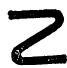
\includegraphics[keepaspectratio]{images/part002_94458643.jpg}}

我们以后将会看到，一般说来，即使 Y = C，也不可能用仅含变量 \(z_{k}\) 的（以 Y 中元素为系数的）多项式一致逼近 f。

推论 2. 设 X 是局部紧空间，\(\mathcal{C}_0(\mathbf{X})\) 是 X 到 C 中的在无穷远处趋于 0 的连续映射所成的赋范 C-代数。设 A 是 \(\mathcal{C}_0(\mathbf{X})\) 的一个分离 X 的点的子代数，且满足：(i) \(\overline{f} \in \mathbf{A}\) ，只要 \(f \in \mathbf{A}\) ；(ii) 对每个 \(x \in \mathbf{X}\) ，存在 \(f \in \mathbf{A}\) 使 \(f(x) \neq 0\) 。则 A 在 \(\mathcal{C}_0(\mathbf{X})\) 中稠密。

若 \(X'\) 是由 X 添加一个无穷远点 \(\omega\) 而得到的紧空间，则 \(\mathcal{C}_{0}(\mathbf{X})\) 可等同于 \(\mathcal{C}(\mathbf{X};\mathbf{C})\) 中由在 \(\omega\) 处为零的连续映射组成的子空间，\(\mathcal{C}_{0}(\mathbf{X})\) 上的范数由下式定义：

\[
\left| \left| f \right| \right| = \sup _ {x \in \mathbf {X}} | f (x) | = \sup _ {x \in \mathbf {X}'} | f (x) |.
\]

根据命题 7，每个 \(f \in \mathcal{C}_{0}(X)\) 都可用 A 中函数的复系数多项式一致逼近；此外，由于 \(f(\omega) = 0\) ，第 2 号命题 4 的论证表明可设这些多项式无常数项，于是它们属于 A。

命题 7 的另一个应用如下：

命题 8. 设 P 是 \(\mathbf{R}^m\) 到 \(\mathbf{C}\) 中的其周期群包含 \(\mathbf{Z}^m\) 的周期连续映射全体所成之集。则属于 P 的每个函数都可在 \(\mathbf{R}^m\) 中用下列形式的函数的复系数线性组合一致逼近：

\[
(x _ {1}, x _ {2}, \dots , x _ {m}) \rightarrow e (h _ {1} x _ {1} + h _ {2} x _ {2} + \dots + h _ {m} x _ {m}),
\]

其中 \(h_{i}\) 是有理整数（这样的线性组合称为 m 个变量的三角多项式）。

只需注意，P（赋有一致收敛拓扑）典范同构于紧空间 \(T^{m}\) 到 C 中的所有连续映射所成的空间（第 VII 章，§ 1，第 6 号），并对 \(T^{m}\) 到 C 中的与 m 个映射 \((x_{1}, x_{2}, \ldots, x_{m}) \to e(x_{i}) \quad (1 \leqslant i \leqslant m)\) (即 \(R^{m}\) 到 C 中的映射)相对应的映射所成之集应用命题 7。

\ExerciseGroupsStart

